\documentclass{article}
	\usepackage[utf8]{inputenc}
	\usepackage{float}
	\usepackage{pdfpages}
	\usepackage[T1]{fontenc}
	\usepackage{float}
	\usepackage{booktabs}
	\usepackage{multirow}
	\usepackage{ragged2e}
	\usepackage{makecell}
	\renewcommand{\theadfont}{\small\bfseries}
	\usepackage{tabularx}
	\usepackage[autolanguage, np]{numprint}
	\newcolumntype{Z}{ >{\centering\arraybackslash}X }
	\usepackage{makecell}
	\usepackage{url}
	\usepackage{siunitx}
	\usepackage{caption}
	\usepackage[framemethod=TikZ]{mdframed}
	\usepackage{tikz, tabularx}
	\usepackage[T1]{fontenc}
	\usepackage{charter}

%%% Document Properties and Packages used 9/20
\usepackage{amsmath}        % math formulas
\usepackage{bm}             % bold math symbols
\usepackage{multicol}       % multiple columns
\usepackage[super]{nth}     % 1st, 2nd, 3rd, 4th
\usepackage{enumitem}       % ordered list (a), (b), (c)
\usepackage{graphicx}		% insert images
\graphicspath{ {./images/} }
\usepackage{geometry}
\geometry{letterpaper, margin=1in, top=0.5in} % small margins
\usepackage{biblatex}		% bibliography
\addbibresource{HW1N1.bib}
%%%%%%%%%%%%%%%%%%%%%%%%%%%%%%%%%%%%%%%%%%%%%%%%%%%%%%%%%%%%%%%%%%%%%%%%%%%%%%%
%%% Code Listing 
\usepackage{listings}
\usepackage{xcolor}

\definecolor{codegreen}{rgb}{0,0.6,0}
\definecolor{codegray}{rgb}{0.5,0.5,0.5}
\definecolor{codepurple}{rgb}{0.58,0,0.82}
\definecolor{backcolour}{rgb}{0.95,0.95,0.92}

\lstdefinestyle{mystyle}{
	backgroundcolor=\color{backcolour},   
	commentstyle=\color{codegreen},
	keywordstyle=\color{magenta},
	numberstyle=\tiny\color{codegray},
	stringstyle=\color{codepurple},
	basicstyle=\ttfamily\footnotesize,
	breakatwhitespace=false,         
	breaklines=true,                 
	captionpos=b,                    
	keepspaces=true,                 
	numbers=left,                    
	numbersep=5pt,                  
	showspaces=false,                
	showstringspaces=false,
	showtabs=false,                  
	tabsize=2
}
\lstset{style=mystyle}
%%%%%%%%%%%%%%%%%%%%%%%%%%%%%%%%%%%%%%%%%%%%%%%%%%%%%%%%%%%%%%%%%%%%%%%%%%%%%%%
\begin{document}
	
	\noindent\textbf{Justine John "JJ" A. Serdoncillo}
	\hfill \textbf{AEM 8202: Fluid Mechanics 2} \\ \hfill \textbf{February 10, 2023}
	
	\begin{center}
		\Large{\textbf{Homework 3}}    
	\end{center}
	
	\section*{Number 2}
		After applying the Boundary Element Method on the circular cylinder, the following plots are made for different values of n for the $\psi_1$ and $\frac{\partial \psi_1}{\partial n}$. It can be seen that even when changing the value of n, the trend of the lines does not change and looks sinusoidal in nature.

		\begin{figure}[H]
			\centering
			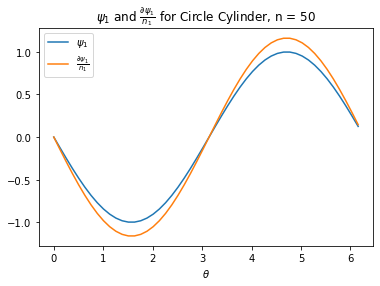
\includegraphics[width=0.6\textwidth]{images/cl50.png}
			\caption{ Plots of $\psi_1$ and $\frac{\partial \psi_1}{\partial n}$ for n=50}
		\end{figure}
	
		\begin{figure}[H]
			\centering
			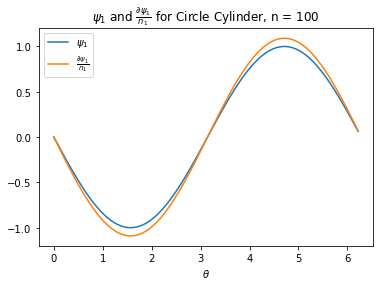
\includegraphics[width=0.6\textwidth]{images/cl100.png}
			\caption{ Plots of $\psi_1$ and $\frac{\partial \psi_1}{\partial n}$ for n=100}
		\end{figure}
	
		\begin{figure}[H]
			\centering
			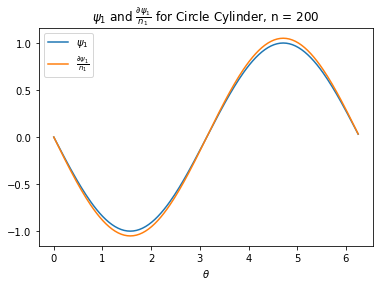
\includegraphics[width=0.6\textwidth]{images/cl200.png}
			\caption{ Plots of $\psi_1$ and $\frac{\partial \psi_1}{\partial n}$ for n=200}
		\end{figure}
	
		It can be seen that as n increase, the partial derivative has its peak getting closer to the 1 value.
	
	\section*{Number 3}
		The following figures below shows the contours of the streamfunction. This corresponds to the streamlines of the flow around the cylinder. 
		
		\begin{figure}[H]
			\centering
			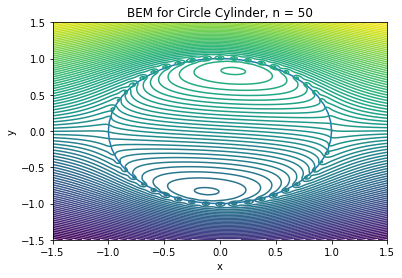
\includegraphics[width=0.6\textwidth]{images/c50v4.png}
			\caption{ Streamlines for n=50}
		\end{figure}
	
		\begin{figure}[H]
			\centering
			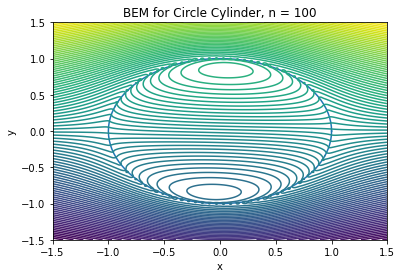
\includegraphics[width=0.6\textwidth]{images/c100v4.png}
			\caption{ Streamlines for n=100}
		\end{figure}
	
		\begin{figure}[H]
			\centering
			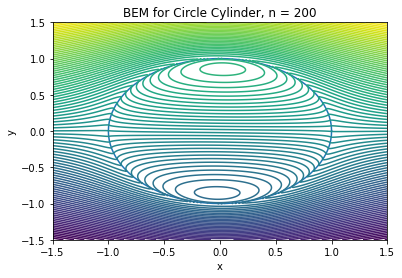
\includegraphics[width=0.6\textwidth]{images/c200v4.png}
			\caption{ Streamlines for n=200}
		\end{figure}
	
		It can be seen that as N increases, the flow near the edge of the cylinder gets more refined. There is not that much of a difference as N increases though quantitatively.

		
	\section*{Number 5}
		After modifying the code to apple to a uniform flow past a 4:1 ellipse parallel and also perpendicular to the flow. The following plots were made below. It can be seen that as n increases, the partial derivative gets smoother. For the horizontal ellipse, the flow doesn't seem to be affected that much because of its streamlines shape. The vertical ellipse changes the flow a lot due to the massive area blocking the flow. There is supposed to be no lines inside so it can be made better next time. 
		
		\begin{figure}[H]
			\centering
			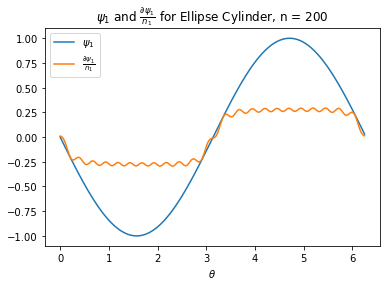
\includegraphics[width=0.6\textwidth]{images/el2001.png}
			\caption{ Plots of $\psi_1$ and $\frac{\partial \psi_1}{\partial n}$ for n=200 Horizontal}
		\end{figure}
	
		\begin{figure}[H]
			\centering
			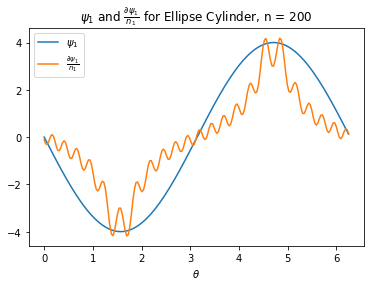
\includegraphics[width=0.6\textwidth]{images/el2002.png}
			\caption{ Plots of $\psi_1$ and $\frac{\partial \psi_1}{\partial n}$ for n=200 Vertical}
		\end{figure}
	
		\begin{figure}[H]
			\centering
			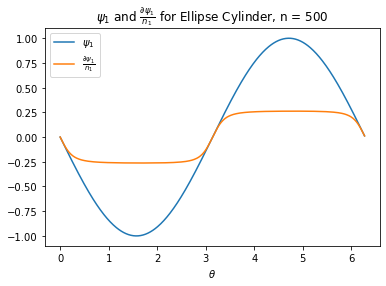
\includegraphics[width=0.6\textwidth]{images/el5001.png}
			\caption{ Plots of $\psi_1$ and $\frac{\partial \psi_1}{\partial n}$ for n=500 Horizontal}
		\end{figure}
		
		\begin{figure}[H]
			\centering
			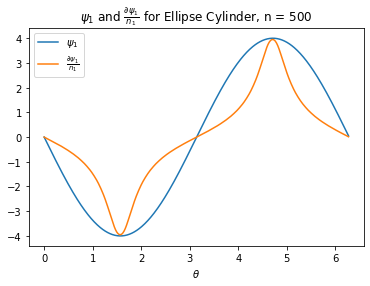
\includegraphics[width=0.6\textwidth]{images/el5002.png}
			\caption{ Plots of $\psi_1$ and $\frac{\partial \psi_1}{\partial n}$ for n=500 Vertical}
		\end{figure}
	
		\begin{figure}[H]
			\centering
			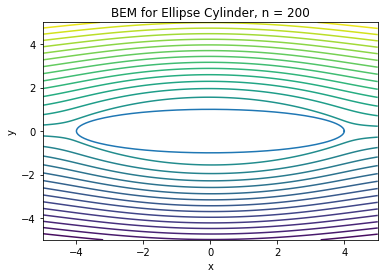
\includegraphics[width=0.6\textwidth]{images/e2001.png}
			\caption{ Streamlines for n=500 Horizontal }
		\end{figure}
		
		\begin{figure}[H]
			\centering
			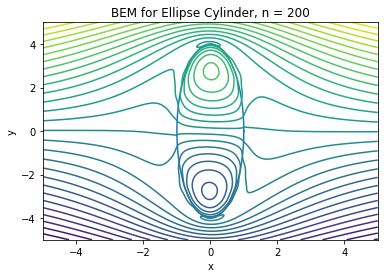
\includegraphics[width=0.6\textwidth]{images/e2002.png}
			\caption{ Streamlines for n=500 Vertical }
		\end{figure}
		
		\begin{figure}[H]
			\centering
			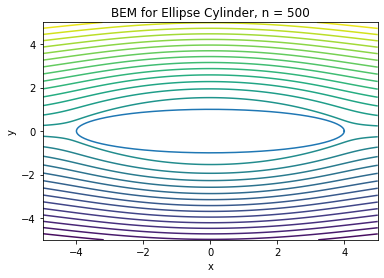
\includegraphics[width=0.6\textwidth]{images/e5001.png}
			\caption{ Streamlines for n=500 Horizontal }
		\end{figure}
		
		\begin{figure}[H]
			\centering
			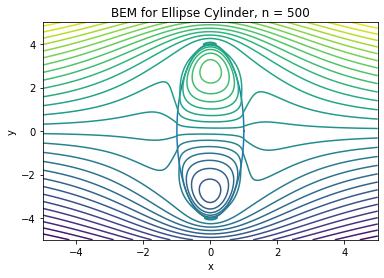
\includegraphics[width=0.6\textwidth]{images/e5002.png}
			\caption{ Streamlines for n=500 Vertical }
		\end{figure}
		
	
		\section*{Appendix)}
			\subsection*{ Python Code for Problems 2,3,5 }
			\lstinputlisting[language=Python]{HW1_v4.py}
	
	
\end{document}
